\documentclass{article}
\usepackage[utf8]{inputenc}

\usepackage[T1]{fontenc}
% \usepackage[czech]{babel}
\usepackage[slovak]{babel}
% \usepackage[english]{babel}
% \usepackage{czech}
% \usepackage{slovak}

\usepackage{mathptmx}  %% volne dostupny font Adobe Times Roman
%  \usepackage[mtbold,mtplusscr,mtpluscal]{mathtime} % komercni matematicky font, dostupne pouze na UMS



\usepackage{longtable,lipsum}


\usepackage{amsmath,amssymb,amsthm}
\usepackage{booktabs}

\usepackage{amsmath}
\usepackage{amssymb}
\usepackage{multicol}
\usepackage{tabularx}
\usepackage{colortbl}
\usepackage{graphicx}
\usepackage[shortlabels]{enumitem}
\usepackage{xcolor}
\usepackage{tcolorbox}
\tcbuselibrary{breakable}
\definecolor{light-gray}{gray}{0.95}

\newcounter{seminar}
\newcounter{problem}
\newcommand{\seminar}[1]{
  \clearpage
  \setcounter{seminar}{#1}
  \setcounter{problem}{0}
  \section*{Seminár #1}
}


\newcommand{\NN}{\mathbb{N}}
\newcommand{\ZZ}{\mathbb{Z}}
\newcommand{\QQ}{\mathbb{Q}}
\newcommand{\RR}{\mathbb{R}}
\newcommand{\kom}{\textbf{Komentár.} }
\newcommand{\ul}[1]{\textbf{Úloha #1.} }
\newcommand{\rie}{\textbf{Riešenie.} }
\newcommand{\rieh}{\textbf{Riešenie*.} }
\newcommand{\ma}{\measuredangle}
\newcommand\todo[1]{\noindent\textcolor{red}{(#1)}}

\newcommand{\source}[1]{
  \def\temp{#1}\ifx\temp\empty
  \else
    [#1]
  \fi
}

\newcommand{\problem}[3]{
  \stepcounter{problem}
  \noindent\textbf{Úloha \theseminar .\theproblem.}
    \source{#1} #2
  \bigskip
}

\begin{document}



\seminar{1}

\seminar{2}

\problem{}{
V Tramtárii chtějí zavést novou základní peněžní jednotku: groš. Ve spojitosti s reformou se vynořila otázka: jaké mají mít hodnoty mince, které připraví mincovna? Staří obyvatelé Tramtárie považovali 3 a 5 za šťastná čísla. Proto přední historik navrhl, aby se omezili na ražení tří- a pětigrošových mincí. Svůj návrh zdůvodňoval takhle: tří- a pětigrošovými mincemi je možné vyplatit jakoukoliv celočíselnou sumu, a to téměř vždy přesně, bez vrácení. Ten, kdo peníze dostává, musí něco vrátit jenom tehdy, když je vyplácená suma 1, 2, 4 nebo 7 grošů. Byla by to pravda?

}{

}



\problem{}{
K návrhu z předchozí úlohy přišel upravující návrh. Jistý občan píše: Uznávám, že tří- a pětigrošovými mincemi je možné popsaným způsobem skutečně zaplatit každou sumu, ale jsou to příliš malé hodnoty. Navrhuji, aby se razily raději pěti- a osmigrošové mince. Je zřejmé -- zdůvodňoval dále --, že všechno, co je možné vyplatit 3 a 5 groši, je možné vyplatit i 5 a 8 groši, vezmeme-li v úvahu možnost vracení peněz. Je taky zřejmé, že od jistého čísla -- tedy v případě větších sum grošů -- ani tady není potřeba mince vracet. Je to skutečně takhle zřejmé?
}{
}



\problem{}{
Diskuse, o které jsme v předchozích dvou úlohách referovali, pokračovala i dál. Byli i tací, kteří pěti- a osmigrošové mince považovali za příliš malé hodnoty a navrhovali větší. Návrhy na dvojice hodnot grošů byly tyto:
\begin{enumerate}[a)]
\item 8 a 13,
\item 21 a 34, 
\item 144 a 233.
\end{enumerate}
Autoři všech tří návrhů tvrdili, že těmito dvojicemi hodnot je možné vyplatit jakékoliv (celočíselné) sumy grošů a když je vyplácená suma dostatečně velká, tak není potřeba ani vracet peníze. Tvrzení kterého z těchto autorů je správné a kterého není?
}{
}



\problem{}{
Tři návrhy, které jsme uvedli v předchozí úloze, nebyly náhodné. Staří obyvatelé uctívali nejen čísla 3 a 5, ale všechna čísla Fibonacciho posloupnosti. Pravděpodobně dospěli až k variacím těchto čísel, protože se objevily i takové návrhy, aby hodnoty dvou mincí byly:
\begin{enumerate}[a)]
\item 2 a 8,
\item 3 a 21, 
\item 21 a 144.
\end{enumerate}
Který z těchto tří návrhů je vhodný na zaplacení jakékoliv (celočíselné) sumy grošů dokonce tak, aby se při dostatečně velké sumě nemuselo nic vrátit?
}{
}

\problem{}{
Diskuse o peněžní reformě v Tramtárii nabývala čím dál větších rozměrů. Mnozí její účastníci tvrdili, že návrhy z úlohy 45 se ukazují býti správnými, protože respektují i pořadí magických čísel, zatímco v úloze 46 jsou neúspěšné, protože toto pořadí nerespektovaly. Jako skutečná bomba proto zapůsobil návrh, aby se vydaly mince v hodnotě 4 a 11 grošů. Ani jedna hodnota se nenacházela mezi \uv{magickými} čísly!  Navzdory tomu autor tvrdil, že i tyto hodnoty splňují potřebné dva požadavky: je možno jimi vyplatit libovolné celočíselné množství grošů a když je tato suma dostatečně velká, ani není potřebné nic vracet. Měl pravdu?}{
}



\problem{}{
Velká diskuse ovšem náhle skončila (právě tehdy, když byla nejživější), protože Národní banka Tramtárie k velkému překvapení oznámila, že zavede dvě platidla: tří- a pětigrošové mince. Kolika různými způsoby je možné jimi vyplatit 49 grošů bez vracení peněz?
}{
}

\seminar{3}
\problem{Lodě}{
Na plánku $7\times 7$ hrajeme hru lodě. Nachází se na něm jedna loď $2\cdot$3. Můžeme vystřelit na libovolné políčko plánku, a když loď zasáhneme, hra končí. Když ne, střílíme znova. Určete nejmenší počet výstřelů, které potřebujeme na to, abychom loď s jistotou zasáhli.
}{}

\seminar{4}

\problem{65-I-3-N1}{
Pro libovolná reálná čísla $x$, $y$ a $z$ dokažte nezápornost hodnoty každého z výrazů
$$x^2+z^2+ y^2-2xyz, \ \ \ \ x^2+ 4y^2+ 3z^2- 2x - 12y - 6z + 13,\ \ \ \  2x^2+ 4y^2+ z^2- 4xy - 2xz$$
a zjistěte rovněž, kdy je dotyčná hodnota rovna nule.
}
{}

\problem{63-I-1-N1-N4}{
\begin{enumerate}[a)]
\item Určete nejmenší hodnotu výrazu $V = 5 + (x - 2)^2$, $x \in \RR$. Pro která $x$ ji výraz nabývá?
\item Určete nejmenší možnou hodnotu výrazu $W = 9-ab$, kde $a$, $b$ jsou reálná čísla splňující podmínku $a + b = 6$. Pro které hodnoty $a$, $b$ je W minimální?
\item  Určete nejmenší možnou hodnotu výrazu $Y = 12-ab$, kde $a$, $b$ jsou reálná čísla splňující podmínku $a + b = 6$. Pro které hodnoty $a$, $b$ je $Y$ minimální?
\item Určete největší možnou hodnotu výrazu $K = 5 + ab$, kde $a$, $b$ jsou reálná čísla splňující podmínku $a + b = 8$. Pro které hodnoty a, b je K maximální?
\end{enumerate}
}{
}

\problem{63-I-1}{
Určete, jaké nejmenší hodnoty může nabýt výraz $V = (a - b)^2 + (b - c)^2 + (c - a)^2$, splňují-li reálná čísla $a$, $b$, $c$ dvojici podmínek
\begin{align*}
a + 3b + c & = 6,\\
-a + b - c & = 2.
\end{align*}
}{
}

\problem{63-S-1}{
Určete, jakých hodnot může nabývat výraz $V = ab + bc + cd + da$, splňují-li reálná čísla $a$, $b$, $c$, d dvojici podmínek
\begin{align*}
2a - 5b + 2c - 5d & = 4, \\
3a + 4b + 3c + 4d & = 6.
\end{align*}
}{
}

\problem{65-I-3}{
Uvažujme výraz
$$2x^2+ y^2 - 2xy + 2x + 4.$$
\begin{enumerate}[a)]
    \item Najděte všechna reálná čísla $x$ a $y$, pro něž daný výraz nabývá své nejmenší hodnoty.
\item Určete všechny dvojice celých nezáporných čísel $x$ a $y$, pro které je hodnota daného výrazu rovna číslu 16.
\end{enumerate}
}{
}

\problem{65-II-1}{
Najděte nejmenší možnou hodnotu výrazu
$$3x^2 - 12xy + y^4,$$
ve kterém $x$ a $y$ jsou libovolná celá nezáporná čísla.
}{
}

\problem{65-I-3-D1}{
 V oboru celých čísel řešte rovnici $x^2+ y^2+ x + y = 4.$
 }{
 }


\seminar{5}

\problem{58-S-1, resp. 65-I-3-D3}{
Dokažte, že pro libovolná nezáporná čísla $a$, $b$, $c$ platí $$(a + bc)(b + ac) \geq ab(c + 1)^2.$$
Zjistěte, kdy nastane rovnost.
}{
}

\problem{66-I-1-N1}{
Dokažte, že pro libovolná reálná čísla $x$, $y$ a $z$ platí nerovnosti
\begin{enumerate}[a)]
\item $2xyz \leq x^2+ y^2z^2$,
\item $(x^2 - y^2)^2\geq 4xy(x - y)^2$.
\end{enumerate}
}{
}

\problem{66-I-1-N2}{
Dokažte, že pro libovolná kladná čísla $a$, $b$ platí nerovnost
$$\frac{a}{b^2}+\frac{b}{a^2}\geq\frac{1}{a}+\frac{1}{b}.$$
}{
}

\problem{62-I-2-N1}{
Dokažte nerovnost
$$\frac{1}{ab}+\frac{1}{cd}\geq \frac{8}{(a+b)(c+d)},$$
pro libovolná kladná čísla $a$, $b$, $c$, $d$.
}{
}

\problem{66-I-1}{
Dokažte, že pro libovolné reálné číslo a platí nerovnost
$$a^2+\frac{1}{a^2 - a + 1}\geq  a + 1.$$
Určete, kdy nastane rovnost.
}{
}

\problem{59-I-5}{
Dokažte, že pro libovolná kladná reálná čísla $a$, $b$ platí
$$\sqrt{ab} \leq \frac{2(a^2 + 3ab + b^2)}{5(a + b)}\leq \frac{a + b}{2},$$
a pro každou z obou nerovností zjistěte, kdy přechází v rovnost.
}{
}

\problem{58-I-6-N3, resp. 62-I-2-N1}{
 Dokažte, že pro libovolná kladná čísla $a$, $b$ a $c$ platí nerovnost
 $$\bigg( a +\frac{1}{b}\bigg)\bigg(b+\frac{1}{c}\bigg) \bigg(c+\frac{1}{a}\bigg)\geq 8$$
a zjistěte, kdy přechází v rovnost.
}{
}

\problem{resp. 59-II-2}{ Dokažte, že pro libovolná čísla $a$, $b$ z intervalu $\langle 1, \infty)$ platí nerovnost
$$(a^2 + 1)(b^2 + 1) - (a - 1)^2 (b - 1) 2 \geq 4,$$
a zjistěte, kdy nastane rovnost.
}{
}

\problem{58-I-6, resp. 62-I-2-N2}{
Dokažte, že pro libovolná různá kladná čísla $a$, $b$ platí
$$\frac{a + b}{2}<\frac{2(a^2+ ab + b^2)}{3(a +b)}<\sqrt{\frac{a^2 + b^2}{2}}.$$
}{}

\seminar{6}

\problem{60-I-1-N1}{
Máme tři čísla se součtem $2 010$, přičemž každé z nich je aritmetickým průměrem zbylých dvou. Jaká jsou to čísla?
}{
}

\problem{60-I-2-N2}{
Máme tři čísla, o nichž víme, že každé z nich je aritmetickým průměrem některých dvou z našich tří čísel. Dokažte, že naše tři čísla jsou stejná
}{
}

\problem{60-I-1}{
Lucie napsala na tabuli dvě nenulová čísla. Potom mezi ně postupně vkládala znaménka plus, mínus, krát a děleno a všechny čtyři příklady správně vypočítala. Mezi výsledky byly pouze dvě různé hodnoty. Jaká dvě čísla mohla Lucie na tabuli napsat?
}{
}

\problem{60-II-1}{
Na tabuli jsou napsána právě tři (ne nutně různá) reálná čísla. Víme, že součet libovolných dvou z nich je tam napsán také. Určete všechny trojice takových čísel.
}{
}

\problem{60-S-1}{
Po okruhu běhají dva atleti, každý jinou konstantní rychlostí. Jestliže běží opačnými směry, potkávají se každých 10 minut, jestliže běží stejným směrem, potkávají se každých 40 minut. Za jakou dobu uběhne okruh rychlejší atlet?
}{
}

\problem{66-I-4-N1}{
 Určete všechny dvojčleny $P(x) = ax + b$, pro které platí $P(2) = 3$ a $P(3) = 2$.
 }{
 }

 \problem{66-I-4-N2}{
Určete všechny trojčleny $P(x) = ax^2+ bx + c$, pro které platí $P(1) = 4$, $P(2) = 9$ a $P(3) =18$.
}{
}

\problem{66-I-4-N3}{
Určete všechny dvojčleny $P(x) = ax + b$ s celočíselnými koeficienty $a$ a $b$, pro které
platí $P(1) < P(2)$ a $P(1)^2+ P(2)^2= 5$.
}{
}

\problem{66-I-4-D2}{
Koeficienty $a$, $b$, $c$ trojčlenu $P(x) = ax^2+ bx + c$ jsou reálná čísla, přitom každá ze tří jeho hodnot $P(1)$, $P(2)$ a $P(3)$ je celým číslem. Plyne odtud, že také čísla $a$, $b$, $c$ jsou celá, nebo je nutně celé aspoň některé z nich (které)?
}{
}

\problem{59-S-3}{
Najděte všechny dvojice nezáporných celých čísel $a$, $b$, pro něž platí $$a^2 +b+2 = a+b^2$$.
}{
}

\problem{66-I-4}{
Nalezněte všechny trojčleny $P(x) = ax^2 +bx+c$ s celočíselnými koeficienty $a$, $b$ a $c$, pro které platí $P(1) < P(2) < P(3)$ a zároveň  $$(P(1))^2+(P(2))^2+  (P(3))^2= 22.$$
}{
}

\problem{62-II-3}{
Najděte všechny dvojice celých kladných čísel $a$ a $b$, pro něž je číslo $a^2 + b$ o $62$ větší než číslo $b^2 + a$.
}{
}

\problem{60-I-1-D1}{
Nechť $n$ je přirozené číslo větší než 2. Máme $n$ čísel se součtem $n$, přičemž každé z nich je aritmetickým průměrem ostatních čísel. Jaká jsou to čísla?
}{
}

\seminar{7}

\problem{Hol10}{
Nechť je $N$ pěticiferné kladné číslo takové, že $N=\overline{a679b}$. Pokud je $N$ dělitelné 72, určete první cifru $a$ a poslední cifru $b$.
}{
}

\problem{66-I-2-N1}{
Dokažte, že v nekonečné řadě čísel
$$1 \cdot 2 \cdot 3, \ \ 2 \cdot 3 \cdot 4, \ \ 3 \cdot 4 \cdot 5, \ \ 4 \cdot 5 \cdot 6, \dots ,$$
je číslo první dělitelem všech čísel dalších.
}{
}

\problem{63-I-5-N1}{
Dokažte, že pro každé přirozené $n$ je číslo $n^3 + 2n$ dělitelné třemi.
}{
}

\problem{63-I-5-N2}{
Dokažte, že pro každé liché číslo $n$ je číslo $n^2 - 1$ dělitelné osmi.
}{
}

\problem{63-I-5-N3-N4, resp. 55-I-1}{
\begin{enumerate}[a)]
    \item Dokažte, že pro všechna celá kladná čísla $n$ je rozdíl $n^6 - n^2$ dělitelný šedesáti.
    \item Určete všechna kladná celá čísla $m$, pro která je rozdíl $m^6 - m^2$ dělitelný číslem 120.
\end{enumerate}
}{
}

\problem{59-II-1, resp. 66-I-2-D2}{
Dokažte, že pro libovolná celá čísla $n$ a $k$ větší než 1 je číslo $n^{k+2}-n^k$ dělitelné dvanácti.
}{
}

\problem{58-S-3}{
 Jestliže jistá dvě přirozená čísla ve stejném pořadí sečteme, odečteme, vydělíme a vynásobíme a všechny čtyři výsledky sečteme, dostaneme $2 009$. Určete tato dvě čísla.
}{
}

\problem{66-I-2-N2}{
Najděte všechna celá $d >1$, při nichž hodnoty výrazů $U(n) = n^3+ 17n^2 - 1$ a $V (n)= n^3+ 4n^2+ 12$ dávají při dělení číslem $d$ stejné zbytky, ať je celé číslo $n$ zvoleno jakkoli.
}{
}

\problem{66-I-2-D1}{
 Pro která přirozená čísla $n$ není výraz $V (n) = n^4+ 11n^2 - 12$ násobkem osmi?
}{
}

\problem{66-I-2}{
Najděte největší přirozené číslo $d$, které má tu vlastnost, že pro libovolné přirozené číslo $n$ je hodnota výrazu
$$V (n) = n^4+ 11n^2 - 12$$
dělitelná číslem $d$.
}{
}

\problem{66-S-2}{
Označme $M$ množinu všech hodnot výrazu $V (n) = n^ 4 + 11n^2 - 12$, kde $n$ je liché přirozené číslo. Najděte všechny možné zbytky při dělení číslem 48, které dávají prvky množiny $M$.
}{
}

\problem{60-I-2}{
Dokažte, že výrazy $23x + y$, $19x + 3y$ jsou dělitelné číslem $50$ pro stejné dvojice přirozených čísel $x$, $y$.
}{
}


\seminar{8}

\problem{61-I-3-N1}{
 Určete, pro která přirozená čísla $a$, $b$ platí $(a, b) = 10$ a zároveň $[a, b] = 150$.
 }{
 }


\problem{60-I-5-N1}{
 Nechť $d$ je největší společný dělitel přirozených čísel $a$ a $b$. Ukažte, že čísla $a/d$ a $b/d$ jsou celá a nesoudělná.
 }{
 }

\problem{60-I-5-N2}{
Dokažte, že pro libovolná přirozená čísla $a$, $b$ platí vztah $[a, b] \cdot (a, b) = ab$.
}{
}

\problem{64-I-5-N4}{
Platí pro každá tři přirozená čísla $a$, $b$, $c$ a jejich největšího společného dělitele $d$ a jejich nejmenší společný násobek $n$ rovnost $abc = nd$?
}{
}

\problem{64-I-5-N5}{
Mají-li přirozená čísla $a$, $b$ největšího společného dělitele $d$, mají stejného největšího společného dělitele i čísla $a$, $b$, $a-b$, $a + b$. Dokažte. Platí stejné tvrzení pro nejmenší
společný násobek?
}{
}

\problem{61-I-3-N4, resp. 50-II-1}{
Najděte všechny dvojice přirozených čísel $a$, $b$, pro které platí $a+b+[a, b]+(a, b) = 50$.
}{
}

\problem{61-S-1}{
Najděte všechny dvojice přirozených čísel $a$, $b$, pro něž platí rovnost množin
$$\{a \cdot [a, b], b \cdot (a, b)\} = \{45,180\}.$$
}{
}

\problem{64-I-5}{
Rozdíl dvou přirozených čísel je $2010$ a jejich největší společný dělitel je $2014$krát menší než jejich nejmenší společný násobek. Určete všechny takové dvojice čísel.
}{
}

\problem{60-I-5-D3}{
Najděte všechny dvojice kladných celých čísel $a$, $b$, pro které má výraz
$$\frac{a}{b}+\frac{14b}{9a}$$
celočíselnou hodnotu.
}{
}

\problem{60-I-5}{
Dokažte, že nejmenší společný násobek $[a, b]$ a největší společný dělitel $(a, b)$ libovolných dvou kladných celých čísel $a$, $b$ splňují nerovnost
$$a \cdot (a, b) + b \cdot [a, b] \geq 2ab.$$
Zjistěte, kdy v této nerovnosti nastane rovnost.
}{
}

\problem{61-I-3}{
Najděte všechny trojice přirozených čísel $a$, $b$, $c$, pro něž platí množinová rovnost
$$\{(a, b), (a, c), (b, c), [a, b], [a, c], [b, c]\}= \{2, 3, 5, 60, 90, 180\},$$
kde $(x, y)$ a $[x, y]$ značí po řadě největší společný dělitel a nejmenší společný násobek čísel $x$ a $y$.
}{
}

\problem{63-S-2}{
Čísla $1, 2, \ldots, 10$ rozdělte do dvou skupin tak, aby nejmenší společný násobek součinu všech čísel první skupiny a součinu všech čísel druhé skupiny byl co nejmenší. Stačí, když uvedete jedno rozdělení a zdůvodníte, proč má požadovanou vlastnost.
}{
}

\seminar{9}

\problem{59-I-6-N1}{%, \todo{Sed61, str. 7}}{
Trojciferné číslo je zakončeno číslicí $4$. Přesuneme-li tuto číslici na první místo (a ostatní dvě číslice ponecháme beze změny), dostaneme číslo, které je o $81$ menší než číslo
původní. Určete původní číslo.
}{
}

\problem{Holton2010, časť 4.1, problem 20}{
Najděte všechna přirozená dvojciferná čísla, která se rovnají dvojnásobku součinu svých cifer.
}{
}

\problem{61-II-2}{
Honza má tři kartičky, na každé je jiná nenulová číslice. Součet všech trojmístných čísel, která lze z těchto kartiček sestavit, je číslo o $6$ větší než trojnásobek jednoho z nich. Jaké číslice jsou na kartičkách?
}{
}

\problem{63-II-1}{
Najděte všechny trojice (ne nutně různých) číslic $a$, $b$, $c$, pro něž pětimístná čísla $\overline{6abc3}$ a $\overline{3abc6}$ jsou v poměru $63 : 36$.
}{
}

\problem{57-I-6-D2, resp. 53-II-4}{
Žáci měli vypočítat příklad $x + y \cdot z$ pro trojmístné číslo $x$ a dvojmístná čísla $y$, $z$. Martin umí násobit a sčítat čísla zapsaná v desítkové soustavě, ale zapomněl na pravidlo přednosti násobení před sčítáním. Proto mu vyšlo sice zajímavé číslo, které se čte stejně zleva doprava jako zprava doleva, správný výsledek byl ale o $2 004$ menší. Určete čísla $x$, $y$, $z$.
}{
}

\problem{58-I-3-N1, resp. 56-S-1}{
Určete počet všech čtyřmístných přirozených čísel, která jsou dělitelná šesti a v jejichž zápisu se vyskytují právě dvě jedničky.
}{
}

\problem{58-I-3-N2, resp. 54-I-5}{
Určete počet všech trojic dvojmístných přirozených čísel $a$, $b$, $c$, jejichž součin abc má zápis, ve kterém jsou všechny číslice stejné. Trojice lišící se pouze pořadím čísel považujeme za stejné, tj. započítáváme je pouze jednou.
}{
}

\problem{59-I-6-N3, resp. 58-I-3}{
Najděte všechna čtyřmístná čísla n, která mají následující tři vlastnosti: V zápise čísla $n$ jsou dvě různé číslice, každá dvakrát. Číslo n je dělitelné sedmi. Číslo, které vznikne obrácením pořadí číslic čísla $n$, je rovněž čtyřmístné a dělitelné sedmi.
}{
}

\problem{59-I-6-N4, resp. 57-I-6}{
Klárka měla na papíru napsáno trojmístné číslo. Když ho správně vynásobila devíti, dostala čtyřmístné číslo, jež začínalo touž číslicí jako číslo původní, prostřední dvě číslice se rovnaly a poslední číslice byla součtem číslic původního čísla. Které čtyřmístné číslo mohla Klárka dostat?
}{
}

\seminar{10}

\problem{}{
Součet velikostí vnitřních úhlů trojúhelníku je roven 180$^\circ$. Dokažte.
}{
}

\problem{66-I-3-N1}{
Připomeňte si, které nerovnosti splňují mezi sebou délky stran libovolného trojúhelníku (a kterým proto říkáme trojúhelníkové). Z nich pak odvoďte známé pravidlo $\alpha < \beta \Rightarrow a < b$ o porovnání velikostí vnitřních úhlů a délek protilehlých stran v libovolném trojúhelníku $ABC$.
}{
}

\problem{63-I-4-N3}{
Dokažte věty:
\begin{enumerate}[a)]
    \item Mají-li dva trojúhelníky stejnou výšku, pak poměr jejich obsahů se rovná poměru délek příslušných základen.
    \item Mají-li dva trojúhelníky shodné základny, pak poměr jejich obsahů se rovná poměru příslušných výšek.
\end{enumerate}
}{
}

\problem{61-I-5-N1}{
Pro obecný trojúhelník $ABC$ o stranách $a$, $b$, $c$ a obsahu $S$ platí pro poloměr $r$ kružnice vepsané vzorec $r = 2S/(a + b + c)$. Dokažte.
}{
}

\problem{anonymous 2}{
Dokažte, že úhlopříčky v rovnoběžníku se navzájem půlí.
}{
}

\problem{58-I-4-N1}{
 Označme $U$ průsečík úhlopříček daného konvexního čtyřúhelníku $ABCD$. Dokažte, že přímky $AB$ a $CD$ jsou rovnoběžné, právě když trojúhelníky $ADU$ a $BCU$ mají stejný obsah.
}{
}

\problem{64-I-4-N1}{
Lichoběžník $ABCD$ má základny o délkách $|AB| = a$, $|CD| = c$, jeho úhlopříčky se protínají v bodě $U$. Jaký je poměr obsahů trojúhelníků $ABU$ a $CDU$?
}{
}

\problem{58-I-2-D2}{
Nechť $k$ je kružnice opsaná pravoúhlému trojúhelníku $ABC$ s přeponou $AB$ délky $c$. Označme $S$ střed strany $AB$ a $D$ a $E$ průsečíky os stran $BC$ a $AC$ s týmž obloukem $AB$ kružnice $k$. Vyjádřete obsah trojúhelníku $DSE$ pomocí délky přepony $c$.
}{
}

\problem{58-I-2-D3}{
Vyjádřete obsah rovnoramenného lichoběžníku $ABCD$ se základnami $AB$ a $CD$ pomocí délek $a$, $c$ jeho základen a délky $b$ jeho ramen.
}{
}

\problem{anonymous 3}{
Užitím vět o podobnosti trojúhelníků a Pythagorovy věty odvoďte Euklidovy věty o odvěsně a výšce pravoúhlého trojúhelníku.
}{
}

\seminar{11}

\problem{66-S-3}{
Pata $P$ výšky z vrcholu $C$ v trojúhelníku $ABC$ dělí stranu $AB$ v poměru $|AP| : |PB| = 1 : 3$. Ve stejném poměru jsou i obsahy čtverců nad jeho stranami $AC$ a $BC$. Dokažte, že trojúhelník $ABC$ je pravoúhlý.
}{
}


\problem{66-I-3}{
Pata výšky z vrcholu $C$ v trojúhelníku $ABC$ dělí stranu $AB$ v poměru $1 : 2$. Dokažte, že při obvyklém označení délek stran trojúhelníku $ABC$ platí nerovnost
$$3|a - b| < c.$$
}{
}

\problem{63-S-3}{
Je dán trojúhelník $ABC$ s pravým úhlem při vrcholu $C$. Středem $I$ kružnice trojúhelníku vepsané vedeme rovnoběžky se stranami $CA$ a $CB$, které protnou přeponu po řadě v bodech $X$ a $Y$ . Ukažte, že platí $|AX|^2 + |BY |^2 = |XY|^2$ .
}{
}

\problem{58-S-2}{
V pravoúhlém trojúhelníku $ABC$ označíme $P$ patu výšky z vrcholu $C$ na přeponu $AB$. Průsečík úsečky $AB$ s přímkou, která prochází vrcholem $C$ a středem kružnice vepsané trojúhelníku $PBC$, označíme $D$. Dokažte, že úsečky $AD$ a $AC$ jsou shodné.
}{
}

\problem{64-I-4}{
Označme $E$ střed základny $AB$ lichoběžníku $ABCD$, v němž platí $|AB| : |CD| = 3 : 1$. Úhlopříčka $AC$ protíná úsečky $ED$, $BD$ po řadě v bodech $F$, $G$. Určete postupný poměr $|AF| : |FG| : |GC|$.
}{
}

\problem{63-I-4}{
Ve čtverci $ABCD$ označme $K$ střed strany $AB$ a $L$ střed strany $AD$. Úsečky $KD$ a $LC$ se protínají v bodě $M$ a rozdělují čtverec na dva trojúhelníky a dva čtyřúhelníky. Vypočtěte jejich obsahy, jestliže úsečka $LM$ má délku 1\,cm.
}{
}

\problem{65-II-3}{
V pravoúhlém lichoběžníku $ABCD$ s pravým úhlem u vrcholu $A$ základny $AB$ je bod $K$ průsečíkem výšky $CP$ lichoběžníku s jeho úhlopříčkou $BD$. Obsah čtyřúhelníku $APCD$ je polovinou obsahu lichoběžníku $ABCD$. Určete, jakou část obsahu trojúhelníku $ABC$ zaujímá trojúhelník $BCK$.
}{
}

\problem{58-I-2}{
Pravoúhlému trojúhelníku $ABC$ s přeponou $AB$ je opsána kružnice. Paty kolmic z bodů $A$, $B$ na tečnu k této kružnici v bodě $C$ označme $D$, $E$. Vyjádřete délku úsečky $DE$ pomocí délek odvěsen trojúhelníku $ABC$.
}{
}

\problem{58-II-2}{
V pravoúhlém trojúhelníku $ABC$ označíme $P$ patu výšky z vrcholu $C$ na přeponu $AB$ a $D$, $E$ středy kružnic vepsaných po řadě trojúhelníkům $APC$, $CPB$. Dokažte, že střed kružnice vepsané trojúhelníku $ABC$ je průsečíkem výšek trojúhelníku $CDE$.
}{
}


\seminar{12}

\problem{57-S-2, resp. 62-I-6-N1}{
V daném rovnoběžníku $ABCD$ je bod $E$ střed strany $BC$ a bod $F$ leží uvnitř strany $AB$. Obsah trojúhelníku $AFD$ je 15\,cm$^2$ a obsah trojúhelníku $FBE$ je 14\,cm$^2$. Určete obsah čtyřúhelníku $FECD$.
}{
}

\problem{62-II-2}{
Uvnitř rovnoběžníku $ABCD$ je dán bod $K$ a v pásu mezi rovnoběžkami $BC$ a $AD$ v polorovině opačné k $CDA$ je dán bod $L$. Obsahy trojúhelníků $ABK$, $BCK$, $DAK$ a $DCL$ jsou $S_{ABK} = 18$\,cm$^2$, $S_{BCK} = 8$\,cm$^2$, $S_{DAK} = 16$\,cm$^2$, $S_{DCL} = 36$\,cm$^2$. Vypočítejte obsahy trojúhelníků $CDK$ a $ABL$.
}{
}

\problem{64-S-2}{
Označme $K$ a $L$ po řadě body stran $BC$ a $AC$ trojúhelníku $ABC$, pro které platí $|BK| =\frac{1}{3}|BC|$, $|AL| =\frac{1}{3}|AC|$. Nechť $M$ je průsečík úseček $AK$ a $BL$. Vypočítejte poměr obsahů trojúhelníků $ABM$ a $ABC$.
}{
}

\problem{64-II-3}{
Je dán lichoběžník $ABCD$ se základnami $AB$, $CD$, přičemž $2|AB| = 3|CD|$.
\begin{enumerate}[a)]
\item Najděte bod $P$ uvnitř lichoběžníku tak, aby obsahy trojúhelníků $ABP$ a $CDP$ byly v poměru $3 : 1$ a rovněž obsahy trojúhelníků $BCP$ a $DAP$ byly v poměru $3 : 1$.
\item Pro nalezený bod $P$ určete postupný poměr obsahů trojúhelníků $ABP$, $BCP$, $CDP$ a $DAP$.
\end{enumerate}
}{
}

\problem{62-I-6}{
Uvnitř pravidelného šestiúhelníku $ABCDEF$ s obsahem 30\,cm$^2$ je zvolen bod $M$. Obsahy trojúhelníků $ABM$ a $BCM$ jsou po řadě 3\,cm$^2$ a 2\,cm$^2$. Určete obsahy trojúhelníků $CDM$, $DEM$, $EFM$ a $FAM$.
}{
}

\problem{65-I-4}{
Uvnitř stran $AB$, $AC$ daného trojúhelníku $ABC$ jsou zvoleny po řadě body $E$, $F$, přičemž $EF \parallel BC$. Úsečka $EF$ je pak rozdělena bodem $D$ tak, že platí
$$p = |ED| : |DF| = |BE| : |EA|.$$
\begin{enumerate}[a)]
\item Ukažte, že poměr obsahů trojúhelníků $ABC$ a $ABD$ je pro $p = 2 : 3$ stejný jako pro $p = 3 : 2$.
\item Zdůvodněte, proč poměr obsahů trojúhelníků $ABC$ a $ABD$ má hodnotu nejméně 4.
\end{enumerate}
}{
}


\seminar{13}

\problem{57-II-1}{
Trojúhelník $ABC$ splňuje při obvyklém značení délek stran podmínku $a \leq b \leq c$. Vepsaná kružnice se dotýká stran $AB$, $BC$ a $AC$ po řadě v bodech $K$, $L$ a $M$. Dokažte, že z úseček $AK$, $BL$ a $CM$ lze sestrojit trojúhelník, právě když platí $b + c < 3a.$
}{
}

\problem{61-S-2}{
Označme $S$ střed základny $AB$ daného rovnoramenného trojúhelníku $ABC$. Předpokládejme, že kružnice vepsané trojúhelníkům $ACS$, $BCS$ se dotýkají přímky $AB$ v bodech, které dělí základnu $AB$ na tři shodné díly. Vypočtěte poměr $|AB| : |CS|$.
}{
}

\problem{62-S-1}{
Danému rovnostrannému trojúhelníku vepišme a opišme kružnice. Označme $S$ obsah vzniklého mezikruží a $T$ obsah kruhu, jehož průměr je shodný s délkou strany daného trojúhelníku. Který z obsahů $S$, $T$ je větší? Svou odpověď zdůvodněte.
}{
}

\problem{61-I-5}{
Je dán rovnoramenný trojúhelník se základnou délky $a$ a rameny délky $b$. Pomocí nich vyjádřete poloměr $R$ kružnice opsané a poloměr $r$ kružnice vepsané tomuto trojúhelníku. Pak ukažte, že platí $R\geq 2r$, a zjistěte, kdy nastane rovnost.
}{
}

\problem{63-I-2}{
V rovině jsou dány body $A$, $P$, $T$ neležící v přímce. Sestrojte trojúhelník $ABC$ tak, aby $P$ byla pata jeho výšky z vrcholu $A$ a $T$ bod dotyku strany $AB$ s kružnicí mu vepsanou. Proveďte diskusi počtu řešení vzhledem k poloze daných bodů.
}{
}

\problem{59-I-4}{
Kružnice $k(S; r)$ se dotýká přímky $AB$ v bodě $A$. Kružnice $l(T; s)$ se dotýká přímky $AB$ v bodě $B$ a protíná kružnici $k$ v krajních bodech $C$, $D$ jejího průměru. Vyjádřete délku a úsečky $AB$ pomocí poloměrů $r$, $s$. Dokažte dále, že průsečík $M$ přímek $CD$, $AB$ je středem úsečky $AB$.
}{
}

\problem{61-I-2}{
Délky stran trojúhelníku jsou v metrech vyjádřeny celými čísly. Určete je, má-li trojúhelník obvod 72\,m a je-li nejdelší strana trojúhelníku rozdělena bodem dotyku vepsané kružnice v poměru $3 : 4$.
}{
}


\seminar{14}

\seminar{15}

\seminar{16}

\seminar{17}

\seminar{18}

\problem{60-II-4}{
Nechť $x$, $y$, $z$ jsou kladná reálná čísla. Ukažte, že čísla $x + y + z - xyz$ a $xy + yz + zx - 3$ nemohou být záporná současně.
}{
}

\problem{61-II-1}{
Pro libovolná reálná čísla $x$, $y$, $z$ taková, že $x < y < z$, dokažte nerovnost
$$x^2 - y^2+ z^2 > (x- y + z)^2.$$
}{
}

\problem{66-II-4}{
Dokažte, že pro všechna kladná reálná čísla $a \leq b \leq c$ platí:
$$(-a + b + c)\bigg( \frac{1}{a}+\frac{1}{b}+\frac{1}{c} \bigg)\geq 3.$$
}{
}

\problem{61-I-4}{
Reálná čísla $a$, $b$, $c$, $d$ vyhovují rovnici $ab + bc + cd + da = 16$.
\begin{enumerate}[a)]
\item Dokažte, že mezi čísly $a$, $b$, $c$, $d$ se najdou dvě se součtem nejvýše 4.
\item Jakou nejmenší hodnotu může mít součet $a^2 + b^2 + c^2 + d^2$?
\end{enumerate}
}{
}

\problem{62-I-2}{
Pro kladná reálná čísla $a$, $b$, $c$, $d$ platí
$$a + b = c + d, \ \ \ \ ad = bc, \ \ \ \ ac + bd = 1.$$
Jakou největší hodnotu může mít součet $a + b + c + d$?
}{
}

\problem{62-I-2-N1}{
Ukažte, že nerovnost $\frac{1}{2}(u + v) =\sqrt{uv}$ mezi aritmetickým a geometrickým průměrem dvou libovolných nezáporných čísel $u$ a $v$ plyne ze zřejmé nerovnosti $(a - b)^2= 0$ vhodnou volbou hodnot $a$ a $b$.}{}

\problem{62-I-2-N1, resp. B-55-S-1}{
 Dokažte, že pro libovolná kladná čísla $a$, $b$ a $c$ platí nerovnost
$$\bigg( a +\frac{1}{b} \bigg) \bigg(b +\frac{1}{c} \bigg) \bigg( c + \frac{1}{a} \bigg)\geq 8.$$
Zjistěte, kdy nastane rovnost
}{}


\seminar{19}

\problem{59-S-1}{
Zvětšíme-li čitatel i jmenovatel jistého zlomku o 1, dostaneme zlomek o hodnotu 1/20 větší. Provedeme-li s větším zlomkem stejnou operaci, dostaneme zlomek o hodnotu 1/12 větší, než byla hodnota zlomku na počátku. Určete všechny tři zlomky.
}{
}

\problem{59-I-3-N1 a)}{
Určete $\lfloor 0 \rfloor$, $\lfloor 3,5 \rfloor$, $\lfloor 2,1 \rfloor$, $\lfloor-4 \rfloor$, $\lfloor-3,9\rfloor$, $\lfloor- 0,2 \rfloor$. Symbol $\lfloor x \rfloor$ značí největší celé číslo, které není větší než číslo $x$, tzv. dolní celou část reálného čísla $x$.
}{
}

\problem{59-I-3-N1 b)}{
Nechť $a$ je celé číslo a $t \in \langle 0, 1)$. Určete $\lfloor a \rfloor$, $\lfloor a + t \rfloor$, $\lfloor a + \frac{1}{2}t \rfloor$, $\lfloor a - t \rfloor$, $\lfloor a + 2t \rfloor$, $\lfloor a - 2t \rfloor$.
}{
}

\problem{59-I-3}{
Určete všechna reálná čísla $x$, která vyhovují rovnici $4x- 2 \lfloor x \rfloor = 5$.
}{
}

\problem{57-I-3-N1}{
Určete všechna celá čísla $n$, pro která nabývá zlomek $(4n + 27)/(n + 3)$ celočíselné hodnoty.
}{
}

\problem{57-I-3}{
Máme určitý počet krabiček a určitý počet kuliček. Dáme-li do každé krabičky právě jednu kuličku, zbyde nám $n$ kuliček. Když však dáme právě $n$ krabiček stranou, můžeme všechny kuličky rozmístit tak, aby jich v každé zbývající krabičce bylo právě $n$. Kolik máme krabiček a kolik kuliček?}{}

\problem{57-II-4}{
Najděte všechny trojice celých čísel x, y, z, pro něž platí
$$x + y \sqrt{3} + z\sqrt{7} = y + z \sqrt{3} + x \sqrt{7}.$$
}{
}

\problem{64-I-1}{Určete všechny dvojice $(x, y)$ reálných čísel, která vyhovují soustavě rovnic
\begin{align*}
\sqrt{(x + 4)^2} & = 4 - y,\\
\sqrt{(y - 4)^2} & = x + 8.
\end{align*}
}{
}

\problem{59-II-4}{
Určete všechny dvojice reálných čísel $x$, $y$, které vyhovují soustavě rovnic
\begin{align*}
\lfloor x + y \rfloor & = 2 010,\\
\lfloor x \rfloor - y & = p,
\end{align*}
jestliže a) $p = 2$, b) $p = 3$.
}{
}

\problem{64-S-1}{
V oboru reálných čísel řešte soustavu rovnic
\begin{align*}
|1 - x| &= y + 1,\\
|1 + y| & = z - 2,\\
|2 - z| & = x - x^2.
\end{align*}}{}


\seminar{20}

\problem{63-I-3-N2}{
Číslo $n$ je součinem dvou různých prvočísel. Zvětšíme-li menší z nich o 1 a druhé ponecháme, jejich součin se zvětší o 7. Určete číslo $n$.
}{
}

\problem{63-I-3-N4}{
 Číslo $n$ je součinem dvou prvočísel. Zvětšíme-li každé z nich o 1, jejich součin se zvětší o 35. Určete číslo $n$.
}{
}

\problem{63-I-3}{
Číslo $n$ je součinem tří různých prvočísel. Zvětšíme-li dvě menší z nich o 1 a největší ponecháme nezměněno, zvětší se jejich součin o 915. Určete číslo $n$.
}{
}

\problem{64-S-3}{
Najděte nejmenší přirozené číslo $n$ s ciferným součtem 8, které se rovná součinu tří různých prvočísel, přičemž rozdíl dvou nejmenších z nich je 8.
}{
}

\problem{57-S-1}{
Najděte všechny dvojice přirozených čísel $a$, $b$ větších než 1 tak, aby jejich součet i součin byly mocniny prvočísel (s kladnými celočíselnými mocniteli).
}{
}

\problem{65-I-1-D2, resp. 55-II-4}{
Najděte všechny dvojice prvočísel $p$ a $q$, pro které platí $p + q^2= q + 145p^2$.
}{
}

\problem{62-I-5, resp. 66-I-2-D4}{
Určete všechna celá čísla $n$, pro něž $2n^3 - 3n^2+ n + 3$ je prvočíslo.
}{
}

\problem{\todo{MŘMUI, 2.3, str, 174}}{
Nalezněte všechna prvočísla, která jsou současně součtem i rozdílem dvou vhodných prvočísel.
}{
}

\problem{Thiele, str. 95}{
Najděte celočíselná řešení rovnice $$\frac{1}{x}+\frac{1}{y}=\frac{1}{p},$$
kde $p$ je pevně dané prvočíslo.}{
}

\problem{65-I-1}{
Najděte všechny možné hodnoty součinu prvočísel $p$, $q$, $r$, pro která platí
$$p^2 - (q + r)^2= 637.$$
}{
}

\seminar{21}

\problem{65-II-4}{
Adam s Bárou hrají se zlomkem
$$\frac{10a + b}{10c + d}$$
takovou hru na čtyři tahy: Hráči střídavě nahrazují libovolné z dosud neurčených písmen $a$, $b$, $c$, $d$ nějakou číslicí od 1 do 9. Bára vyhraje, když výsledný zlomek bude roven buď celému číslu, nebo číslu s konečným počtem desetinných míst; jinak vyhraje Adam (například když vznikne zlomek $\frac{11}{29}$). Začíná-li Adam, jak má hrát Bára, aby zaručeně vyhrála? Začíná-li Bára, je možné poradit Adamovi tak, aby vždy vyhrál?
}{
}

\problem{57-I-1-N1}{
Jsou-li $m$, $k$ a $\sqrt[k]{m}$ celá čísla větší než 1, pak v rozkladu čísla $m$ na prvočinitele se každé prvočíslo vyskytuje v mocnině, jejíž mocnitel je násobkem čísla $k$. Dokažte.
}{
}

\problem{57-I-1}{
Určete nejmenší přirozené číslo $n$, pro něž i čísla $\sqrt{2n}$, $\sqrt[3]{3n}$, $\sqrt[5]{5n}$ jsou přirozená.
}{
}

\problem{60-II-2}{
Najděte všechna kladná celá čísla $n$, pro která je číslo $n^2 +6n$ druhou mocninou celého
čísla.
}{
}

\problem{66-II-1}{
Najděte všechny mnohočleny $P(x) = ax^2 + bx + c$ s celočíselnými koeficienty splňující
$$1 < P(1) < P(2) < P(3) \ \ \ \  \text{a zároveň} \ \ \ \ \frac{P(1) \cdot P(2) \cdot P(3)}{4}= 17^2.$$
}{
}

\problem{64-II-1}{
Celá čísla od 1 do 9 rozdělíme libovolně do tří skupin po třech a pak čísla v každé skupině mezi sebou vynásobíme.
\begin{enumerate}[a)]
\item Určete tyto tři součiny, jestliže víte, že dva z nich se rovnají a jsou menší než třetí součin.
\item Předpokládejme, že jeden ze tří součinů, který označíme $S$, je menší než dva ostatní součiny (které mohou být stejné). Najděte největší možnou hodnotu $S$.
\end{enumerate}
}{
}

\problem{65-I-5-N1, resp. 58-I-5}{
Z množiny $\{1, 2, 3, \ldots , 99\}$ vyberte co největší počet čísel tak, aby součet žádných dvou vybraných čísel nebyl násobkem jedenácti. Vysvětlete, proč zvolený výběr má požadovanou vlastnost a proč žádný výběr většího počtu čísel nevyhovuje.
}{
}

\problem{64-I-6}{
Najděte nejmenší přirozené číslo $n$ takové, že v zápise čísla $\sqrt{n}$ následují bezprostředně za desetinnou čárkou dvě devítky.}{}


\seminar{22}

\problem{57-I-2}{
Čtyřúhelníku $ABCD$ je vepsána kružnice se středem $S$. Určete rozdíl $|\ma ASD | - |\ma CSD |$, jestliže $|\ma ASB | - |\ma BSC | = 40^\circ$.
}{
}

\problem{61-II-3}{
Nechť $E$ je střed strany $CD$ rovnoběžníku $ABCD$, ve kterém platí $2|AB| = 3|BC|$. Dokažte, že pokud lze do čtyřúhelníku $ABCE$ vepsat kružnici, dotýká se tato kružnice strany $BC$ v jejím středu.
}{
}

\problem{59-II-3}{
Je dána kružnice $k$ se středem $S$. Kružnice $l$ má větší poloměr než kružnice $k$, prochází jejím středem a protíná ji v bodech $M$ a $N$. Přímka, která prochází bodem $N$ a je rovnoběžná s přímkou $MS$, vytíná na kružnicích tětivy $NP$ a $NQ$. Dokažte, že trojúhelník $MPQ$ je rovnoramenný.
}{
}

\problem{60-I-3, \todo{fixnúť obrázok v slovenskom zadaní}}{
Máme čtverec $ABCD$ se stranou délky 1\,cm. Body $K$ a $L$ jsou středy stran $DA$ a $DC$. Bod $P$ leží na straně $AB$ tak, že $|BP| = 2|AP |$. Bod $Q$ leží na straně $BC$ tak, že $|CQ| = 2|BQ|$. Úsečky $KQ$ a $PL$ se protínají v bodě $X$. Obsahy čtyřúhelníků $APXK$, $BQXP$, $QCLX$ a $LDKX$ označíme postupně $S_A$, $S_ B$, $S_C$, $S_D$ \todo{(obr. 1)}.
\begin{enumerate}[a)]
\item Dokažte, že $S_B = S_D$.
\item Vypočtěte rozdíl S$_C - S_A$.
\item Vysvětlete, proč neplatí $S_A + S_C = S_B + S_D$.
\end{enumerate}
\begin{center}
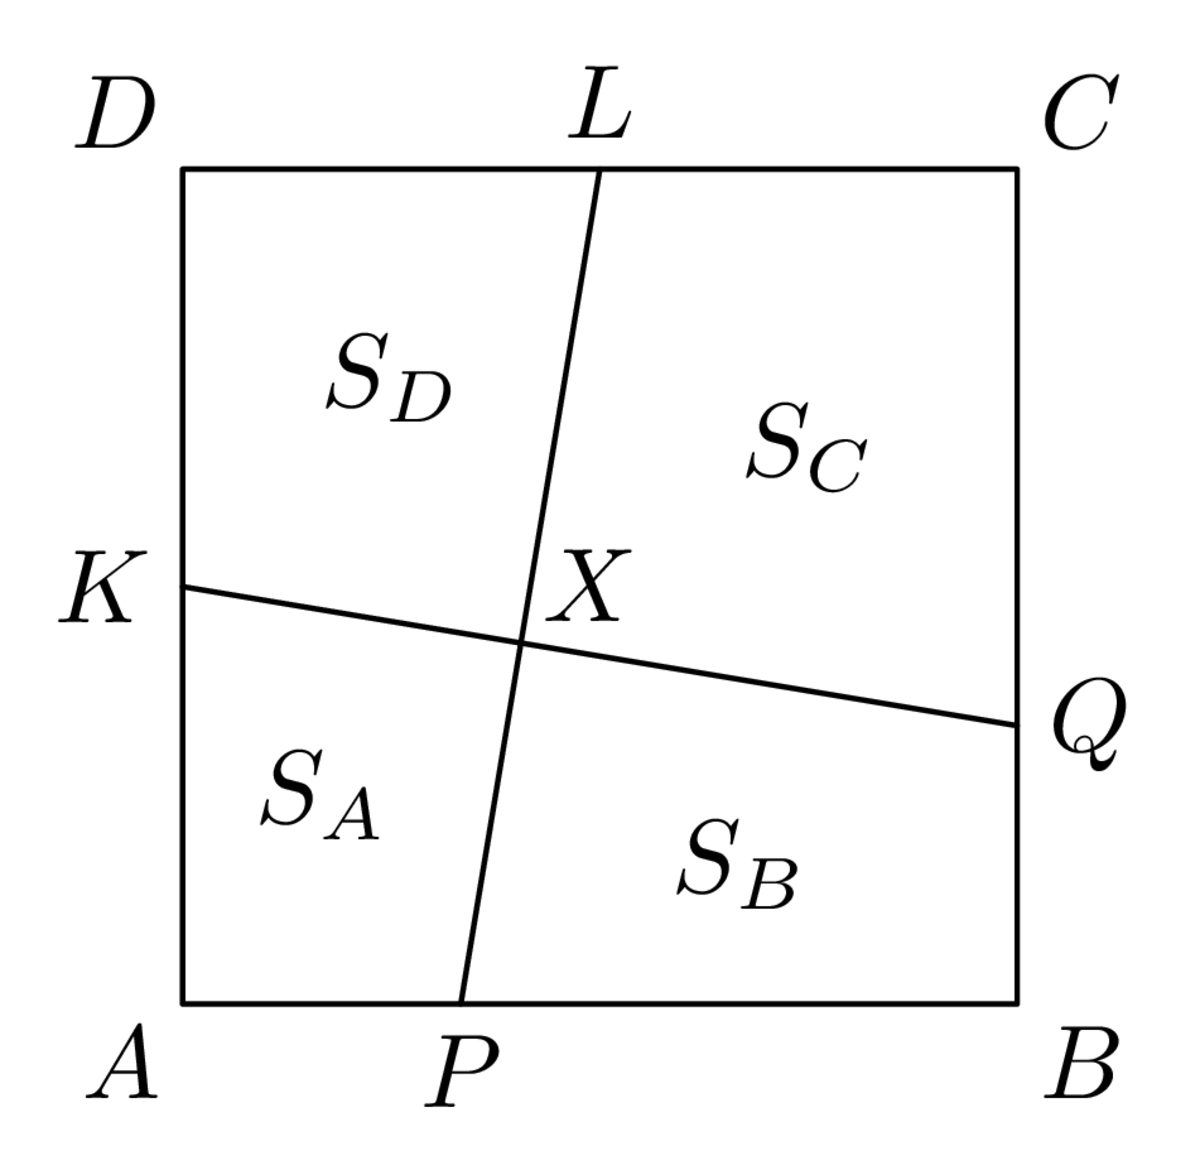
\includegraphics{images/60D31}
\end{center}
}{
}

\problem{66-I-5-první část}{
Označíme-li $X$ a $Y$ po řadě středy základen $RS$ a $TU$, pak na úsečce $XY$ leží průsečík $P$ úhlopříček $RT$ a $SU$, a to tak, že $|PX| : |PY | = |RS| : |TU|$. Na přímce $XY$ leží rovněž průsečík $Q$ prodloužených ramen $RU$ a $ST$, a to tak, že $|QX| : |QY | = |RS| : |TU|$. Dokažte.
}{
}

\problem{66-I-5}{
V daném trojúhelníku $ABC$ zvolme uvnitř strany $AC$ body $K$, $M$ a uvnitř strany $BC$ body $L$, $N$ tak, že
$$|AK| = |KM| = |MC|, \ \ \ \ |BL| = |LN| = |NC|.$$
Dále označme $E$ průsečík úhlopříček lichoběžníku $ABLK$, $F$ průsečík úhlopříček lichoběžníku $KLNM$ a $G$ průsečík úhlopříček lichoběžníku $ABNM$. Dokažte, že body $E$, $F$ a $G$ leží na těžnici z vrcholu $C$ trojúhelníku $ABC$, a určete poměr $|GF| : |EF|$.
}{
}


\seminar{23}

\problem{66-II-3}{
Dokažte, že obdélník o rozměrech $32 \times 120$ lze zakrýt sedmi shodnými čtverci o straně 30.
}{
}

\problem{60-S-2}{
Je dán čtverec se stranou délky 6\,cm. Najděte množinu středů všech příček čtverce, které ho dělí na dva čtyřúhelníky, z nichž jeden má obsah 12\,cm$^2$. (Příčkou čtverce rozumíme úsečku, jejíž krajní body leží na stranách čtverce.)
}{
}

\problem{65-S-2}{
V kružnici o středu $S$ sestrojíme průměr $AB$ a libovolnou k němu kolmou tětivu $CD$. Zdůvodněte, proč je obvod trojúhelníku $ACD$ menší než dvojnásobek obvodu trojúhelníku $SBC$.
}{
}

\problem{59-S-2}{
Kružnice $k(S; 6 cm)$ a $l(O; 4 cm)$ mají vnitřní dotyk v bodě $B$. Určete délky stran trojúhelníku $ABC$, kde bod $A$ je průsečík přímky $OB$ s kružnicí $k$ a bod $C$ je průsečík kružnice $k$ s tečnou z bodu $A$ ke kružnici $l$.
}{
}

\problem{63-II-4}{
Je dán konvexní čtyřúhelník $ABCD$ s bodem $E$ uvnitř strany $AB$ tak, že platí $|\ma ADE| = |\ma DEC| = |\ma ECB|$. Obsahy trojúhelníků $AED$ a $CEB$ jsou po řadě 18\,cm$^2$ a 8\,cm$^2$ . Určete obsah trojúhelníku $ECD$.
}{
}


\seminar{24}


\seminar{25}

\problem{66-II-2}{
Čtvercovou tabulku $6 \times 6$ zaplníme všemi celými čísly od 1 do 36.
\begin{enumerate}[a)]
\item Uveďte příklad takového zaplnění tabulky, kdy součet každých dvou čísel ve stejném řádku či ve stejném sloupci je větší než 11.
\item Dokažte, že při libovolném zaplnění tabulky se v některém řádku nebo sloupci najdou dvě čísla, jejichž součet nepřevyšuje 12.
\end{enumerate}
}{
}

\problem{62-I-1-N1}{
Kobylka skáče po úsečce délky 10\,cm a to skoky o 1\,cm nebo o 2\,cm (vždy stejným směrem). Kolika způsoby se může dostat z jednoho krajního bodu úsečky do druhého?
}{
}

\problem{62-I-1-N2 \todo{fixnúť číslovanie slovenskej verzie, je tam teraz I-2}}{
Skřítek se pohybuje v tabulce $10 \times 15$ skoky o jedno políčko nahoru nebo o jedno políčko doprava. Kolika různými cestami se může dostat z levého dolního do pravého horního políčka?
}{
}

\problem{64-II-2}{
V jednom poli šachovnice $8\times 8$ je napsáno \uv{$-$} a v ostatních polích \uv{+}. V jednom kroku můžeme změnit na opačná zároveň všechna čtyři znaménka v kterémkoli čtverci $2 \times 2$ na šachovnici. Rozhodněte, zda po určitém počtu kroků může být na šachovnici obou znamének stejný počet.
}{
}

\problem{64-I-3-N3}{
Simona a Lenka hrají hru. Pro dané celé číslo $k$ takové, že $0 \leq k \leq 9$, vybere Simona $k$ políček šachovnice $3 \times 3$ a na každé z nich napíše číslo 1, na ostatní políčka napíše číslo 0. Lenka pak šachovnici nějakým způsobem pokryje třemi triminovými kostkami, \todo{tj.} kostkami tvaru $3 \times 1$, a čísla pod jejími políčky vynásobí. Je-li počet kostek se součinem 0 lichý, vyhrává Simona, jinak vyhrává Lenka. V závislosti na $k$ určete, kolikaprocentní vítěznou strategii má Simona.
}{
}

\problem{61-I-6-N1}{
Na hrací desce $m \times n$ tvořené bílými čtvercovými poli se Markéta a Tereza střídají v tazích jedním kamenem při následující hře. Nejprve Markéta umístí kámen na libovolné pole a toto pole obarví modře. Dále vždy hráčka, která je na tahu, provede s kamenem skok na pole, které je dosud bílé, a toto pole obarví modře. Přitom skokem rozumíme obvyklý tah šachovou věží, tj. přesuny kamene ve směru řádků nebo ve směru sloupců hrací desky (o libovolný počet polí). Hráčka, která je na řadě a již nemůže táhnout, prohrává. Postupně pro $n = 4, 5, 6$ rozhodněte, která z hráček může hrát tak, že vyhraje nezávisle na tazích druhé hráčky.
}{
}

\problem{62-I-1}{
Čtvercová tabulka je rozdělena na $16 \times 16$ políček. Kobylka se po ní pohybuje dvěma směry: vpravo nebo dolů, přičemž střídá skoky o dvě a o tři políčka (to jest žádné dva po sobě jdoucí skoky nejsou stejně dlouhé). Začíná skokem délky dva z levého horního políčka. Kolika různými cestami se může kobylka dostat na pravé dolní políčko? (Cestou rozumíme posloupnost políček, na která kobylka skočí.)
}{
}

\problem{61-I-6}{
Na hrací desce $n \times n$ tvořené bílými čtvercovými poli se Markéta a Tereza střídají v tazích jedním kamenem při následující hře. Nejprve Markéta umístí kámen na libovolné pole a toto pole obarví modře. Dále vždy hráčka, která je na tahu, provede s kamenem skok na pole, které je dosud bílé, a toto pole obarví modře. Přitom skokem rozumíme obvyklý tah šachovým jezdcem, tj. přesun kamene o dvě pole svisle nebo vodorovně a současně o jedno pole v druhém směru. Hráčka, která je na řadě a již nemůže táhnout, prohrává. Postupně pro $n = 4, 5, 6$ rozhodněte, která z hráček může hrát tak, že vyhraje nezávisle na tazích druhé hráčky.
}{
}


\seminar{26}

\problem{61-I-6-N2}{
Na tabuli jsou napsána všechna prvočísla menší než 100. Markéta a Tereza se střídají v tazích při následující hře. Nejprve Markéta smaže jedno z prvočísel. Dále vždy hráčka, která je na tahu, smaže jedno z prvočísel, které má s předchozím smazaným prvočíslem jednu shodnou číslici (tak po prvočíslu 3 lze smazat třeba 13 nebo 37). Hráčka, která je na tahu a nemůže již žádné prvočíslo smazat, prohrává. Která z obou hráček může hrát
tak, že vyhraje nezávisle na tazích druhé hráčky?
}{
}

\problem{64-II-4}{
Na tabuli je napsáno prvních $n$ celých kladných čísel. Markéta a Tereza se střídají v tazích při následující hře. Nejprve Markéta smaže jedno z čísel na tabuli. Dále vždy hráčka, která je na tahu, smaže jedno z čísel, které se od předchozího smazaného čísla ani neliší o 1, ani s ním není soudělné. Hráčka, která je na tahu a nemůže již žádné číslo smazat, prohrává. Pro $n = 6$ a pro $n = 12$ rozhodněte, která z hráček může hrát tak, že vyhraje nezávisle na tazích druhé hráčky.
}{
}

\problem{61-I-6-N3}{
Dvě hráčky mají k dispozici pro hru, kterou popíšeme, neomezený počet pětikorun a stůl s kruhovou deskou o průměru 1 metr. Hra probíhá tak, že se hráčky pravidelně střídají v tazích. Nejprve první hráčka položí jednu pětikorunu na prázdný stůl kamkoliv. Dále vždy hráčka, která je na tahu, položí na volnou část stolu další pětikorunu (tak, aby nepřesahovala okraj stolu a aby se dříve uložených pětikorun nejvýše dotýkala). Která z obou hráček může hrát tak, že vyhraje nezávisle na tazích druhé hráčky?
}{
}

\problem{59-I-1}{
\todo{pozisťovať, ako je to tu s kurzívou} Erika a Klárka hrály hru \uv{slovní logik} s těmito pravidly: Hráč $A$ si myslí slovo složené z pěti různých písmen. Hráč $B$ vysloví libovolné slovo složené z pěti různých písmen a hráč $A$ mu prozradí, kolik písmen uhodl na správné pozici a kolik na nesprávné. Písmena považujeme za různá, i když se liší jen háčkem nebo čárkou (například písmena A, Á jsou různá). Kdyby si hráč $A$ myslel například slovo \textit{LOĎKA} a $B$ by vyslovil slovo \textit{KOLÁČ}, odpoví hráč $A$, že jedno písmeno uhodl hráč $B$ na správné pozici a dvě na nesprávné. Zkráceně sdělí \uv{1 + 2}, neboť se opravdu obě slova shodují pouze v písmenu O včetně pozice (druhé zleva) a v písmenech K a L, jejichž pozice jsou odlišné. Erika si myslela slovo z pěti různých písmen a Klárka vyslovila slova \textit{KABÁT}, \textit{STRUK}, \textit{SKOBA}, \textit{CESTA} a \textit{ZÁPAL}. Erika na tato slova v daném pořadí odpověděla $0 + 3$, $0 + 2$, $1 + 2$, $2 + 0$ a $1 + 2$. Zjistěte, jaké slovo si Erika mohla myslet.
}{
}

\problem{63-I-6}{
Šachového turnaje se zúčastnilo 8 hráčů a každý s každým odehrál jednu partii. Za vítězství získal hráč 1 bod, za remízu půl bodu, za prohru žádný bod. Na konci turnaje měli všichni účastníci různé počty bodů. Hráč, který skončil na 2. místě, získal stejný počet bodů jako poslední čtyři dohromady. Určete výsledek partie mezi 4. a 6. hráčem v celkovém pořadí.
}{
}

\problem{63-II-2}{
Šachového turnaje se zúčastnilo 5 hráčů a každý s každým odehrál jednu partii. Za vítězství získal hráč 1 bod, za remízu půl bodu, za prohru žádný bod. Pořadí hráčů v turnaji se určuje podle počtu získaných bodů. Jediným dalším kritériem rozhodujícím o konečném umístění hráčů v případě rovnosti bodů je počet výher (kdo má více výher, je na tom v umístění lépe). V turnaji získali všichni hráči stejný počet bodů. Vojta porazil Petra a o první místo se dělil s Tomášem. Jak dopadla partie mezi Petrem a Martinem?
}{
}

\problem{64-I-3}{
Simona a Lenka hrají hru. Pro dané celé číslo $k$ takové, že $0 \leq k \leq 64$, vybere Simona k políček šachovnice $8\times8$ a každé z nich označí křížkem. Lenka pak šachovnici nějakým způsobem vyplní dvaatřiceti dominovými kostkami. Je-li počet kostek pokrývajících dva křížky lichý, vyhrává Lenka, jinak vyhrává Simona. V závislosti na $k$ určete, která z dívek má vyhrávající strategii.
}{
}

\seminar{27}

\seminar{28}

\problem{}{Kolik karet obsahuje hrací balíček?}{}

\problem{}{Z balíčku vybereme dvě libovolné kartičky. Kolik existuje kartiček takových, aby s původními dvěma tvořily SET, a proč?}{}

\problem{}{Kolik různých SETů (kartičky se v rámci jednotlivých SETů můžou opakovat) se nachází v celém balíčku?}{}

\problem{}{Z balíčku vybereme jednu kartičku. Kolika různých SETů může být tato kartička součástí?}{}

\problem{}{Jakým způsobem je možné ukázat, že se v daném rozložení kartiček na stole nenachází žádný SET?}{}

\problem{}{Je možné SETy nějak kategorizovat? Jak? Kolik různých SETů můžeme v různých kategoriích vytvořit? Umíme správnost našich výpočtů ověřit pomocí předchozích úvah?}{}

\seminar{29}

\problem{B-66-II-1}{
Najděte všechny dvojice přirozených čísel $a$, $b$, pro něž platí
$$a +\frac{66}{a}= b +\frac{66}{b}.$$
}{
}

\problem{B-58-II-1, resp. B-60-1-N4}{
V oboru reálných čísel řešte soustavu rovnic
\begin{align*}
x + y & = 1, \\
x - y & = a, \\
-4ax + 4y & = z^2+ 4
\end{align*}
o neznámých $x$, $y$, $z$ a reálném parametru $a$.}{}

\problem{B-60-S-1}{
V oboru reálných čísel řešte rovnici
$$\sqrt{x + 3} + \sqrt{x} = p$$
s neznámou $x$ a reálným parametrem $p$.
}{
}

\problem{B-58-I-2, resp. B-60-I-1-N3}{
Určete všechny trojice $(x, y, z)$ reálných čísel, pro které platí
\begin{align*}
x^2+ xy & = y^2+ z^2,\\
z^2+ zy & = y^2+ x^2.
\end{align*}
}{
}

\problem{B-60-I-1}{
V oboru reálných čísel vyřešte soustavu
\begin{align*}
\sqrt{x^2 + y^2} & = z + 1,\\
\sqrt{y^2 + z^2} & = x + 1,\\
\sqrt{z^2 + x^2} & = y + 1.
\end{align*}
}{
}

\seminar{30}

\problem{B-57-I-5-N3}{
Najděte všechny dvojice $(a, b)$ reálných čísel, pro něž má každá z rovnic
\begin{align*}
x^2 +(a - 2)x + b - 3 & = 0,\\
x^2 + (a + 2)x + 3b - 5 & = 0
\end{align*}
dvojnásobný kořen.
}{
}

\problem{B-57-I-5}{
Určete všechny dvojice $a$, $b$ reálných čísel, pro něž má každá z kvadratických rovnic
$$ax^2 + 2bx + 1  = 0,\ \ \ \ bx^2 + 2ax + 1 = 0$$
dva různé reálné kořeny, přičemž právě jeden z nich je oběma rovnicím společný.
}{
}

\problem{B-57-II-1}{
Uvažujme dvě kvadratické rovnice
$$x^2-ax - b = 0, \ \ \ \ x^2- bx - a = 0$$
s reálnými parametry $a$, $b$. Zjistěte, jaké nejmenší a jaké největší hodnoty může nabývat součet $a + b$, existuje-li právě jedno reálné číslo $x$, které současně vyhovuje oběma rovnicím. Určete dále všechny dvojice $(a, b)$ reálných parametrů, pro něž uvažovaný součet těchto hodnot nabývá.
}{
}

\problem{B-62-II-1}{
Pro libovolná reálná čísla $p \neq 0$, $q$ a $k \neq \pm 1$ dokažte tvrzení: Rovnice
$$x^2+ px + q = 0$$
má v oboru reálných čísel dva kořeny, z nichž jeden je $k$-násobkem druhého, právě když platí $kp^2 = (k + 1)^2q$.
}{
}

\problem{B-59-I-6}{
Reálná čísla $a$, $b$ mají tuto vlastnost: rovnice $x^2 - ax + b -1 = 0$ má v množině reálných čísel dva různé kořeny, jejichž rozdíl je kladným kořenem rovnice $x^2 -ax++ b + 1 = 0.$
\begin{enumerate}[a)]
\item Dokažte nerovnost $b > 3$.
\item Pomocí $b$ vyjádřete kořeny obou rovnic.
\end{enumerate}
}{
}

\problem{B-64-II-4}{
Na tabuli je seznam čísel $1, 2, 3, 4, 5, 6$ a \uv{rovnice}
$$\frac{\fbox{$\phantom{7}$}}{\fbox{$\phantom{7}$}}x^2+\frac{\fbox{$\phantom{7}$}}{\fbox{$\phantom{7}$}}x + \frac{\fbox{$\phantom{7}$}}{\fbox{$\phantom{7}$}}= 0.$$
Marek s Tomášem hrají následující hru. Nejprve Marek vybere libovolné číslo ze seznamu, napíše je do jednoho z prázdných políček v \uv{rovnici} a číslo ze seznamu smaže. Poté Tomáš vybere některé ze zbývajících čísel, napíše je do jiného prázdného políčka a v seznamu je smaže. Nato Marek provede totéž a nakonec Tomáš doplní tři zbylá čísla na tři zbývající volná políčka v \uv{rovnici}. Marek vyhraje, jestliže vzniklá kvadratická rovnice s racionálními koeficienty bude mít dva různé reálné kořeny, jinak vyhraje Tomáš. Rozhodněte, který z hráčů může vyhrát nezávisle na postupu druhého hráče.
}{
}

\problem{B-57-S-2}{
Určete všechny dvojice $(a, b)$ reálných čísel, pro něž mají rovnice
$$x^2 + (3a + b)x + 4a = 0, \ \ \ \  x^2 + (3b + a)x + 4b = 0$$
společný reálný kořen.
}{
}

\problem{B-59-S-1}{
Určete všechny hodnoty reálných parametrů $p$ a $q$, pro něž má každá z rovnic
$$x(x- p) = 3 + q,  \ \ \ \ x(x + p) = 3 - q$$
v oboru reálných čísel dva různé kořeny, jejichž aritmetický průměr je jedním z kořenů zbylé rovnice.}{}





\seminar{31}

\problem{B-65-I-5-N3}{
Je dána tětiva $AB$ kružnice $k$ se středem v bodě $S$. Na úsečce $AB$ zvolme bod $M$ a průsečík kružnice opsané trojúhelníku $AMS$ s kružnicí $k$ označme $C$. Dokažte, že úhly $MCS$ a $MBS$ jsou shodné.
}{
}

\problem{B-66-II-3}{
V rovině jsou dány kružnice $k$ a $l$, které se protínají v bodech $E$ a $F$. Tečna ke kružnici $l$ sestrojená v bodě $E$ protíná kružnici $k$ v bodě $H$ ($H \neq E$). Na oblouku $EH$ kružnice $k$, který neobsahuje bod $F$, zvolme bod $C$ ($E\neq C \neq H$) a průsečík přímky $CE$ s kružnicí $l$ označme $D$ ($D\neq  E$). Dokažte, že trojúhelníky $DEF$ a $CHF$ jsou podobné.
}{
}

\problem{B-65-II-2}{
Je dána úsečka $AB$, její střed $C$ a uvnitř úsečky $AB$ bod $D$. Kružnice $k(C, |BC|)$ a $m(B, |BD|)$ se protínají v bodech $E$ a $F$. Zdůvodněte, proč je polopřímka $FD$ osou úhlu $AFE$.
}{
}

\problem{B-65-I-5}{
Vrcholy konvexního šestiúhelníku $ABCDEF$ leží na kružnici, přičemž $|AB|= |CD|$. Úsečky $AE$ a $CF$ se protínají v bodě $G$ a úsečky $BE$ a $DF$ se protínají v bodě $H$. Dokažte, že úsečky $GH$, $AD$ a $BC$ jsou navzájem rovnoběžné.
}{
}

\problem{B-58-I-5}{
Trojúhelníku $ABC$ je opsána kružnice $k$. Osa strany $AB$ protne kružnici $k$ v bodě $K$, který leží v polorovině opačné k polorovině $ABC$. Osy stran $AC$ a $BC$ protnou přímku $CK$ po řadě v bodech $P$ a $Q$. Dokažte, že trojúhelníky $AKP$ a $KBQ$ jsou shodné.
}{
}

\seminar{32}

\problem{B-59-II-1}{
Kružnice $l(T; s)$ prochází středem kružnice $k(S; 2 cm)$. Kružnice $m(U; t)$ se vně dotýká kružnic $k$ a $l$, přičemž $US \perp ST$. Poloměry $s$ a $t$ vyjádřené v centimetrech jsou celá čísla. Určete je.
}{
}

\problem{B-66-S-2}{
Na odvěsnách $AC$ a $BC$ daného pravoúhlého trojúhelníku $ABC$ určete po řadě body $K$ a $L$ tak, aby součet
$$|AK|^2 + |KL|^2 + |LB|^2$$
nabýval nejmenší možné hodnoty, a vyjádřete ji pomocí $c = |AB|$.
}{
}

\problem{B-63-S-3}{
Na přímce $a$, na níž leží strana $BC$ trojúhelníku $ABC$, jsou dány body dotyku všech tří mu připsaných kružnic (body $B$ a $C$ nejsou známy). Najděte na této přímce bod dotyku kružnice vepsané.
}{
}

\problem{B-65-I-3}{
V pravoúhlém trojúhelníku $ABC$ s přeponou $AB$ a odvěsnami délek $|AC| = 4$\,cm a $|BC| = 3$\,cm leží navzájem se dotýkající kružnice $k_ 1(S_1; r_1)$ a $k_ 2(S_2; r_2)$ tak, že $k_1$ se dotýká stran $AB$ a $AC$, zatímco $k_2$ se dotýká stran $AB$ a $BC$. Určete nejmenší a největší možnou hodnotu poloměru $r_2$.
}{
}

\problem{B-61-II-3}{
Pravoúhlému trojúhelníku $ABC$ je vepsána kružnice, která se dotýká přepony $AB$ v bodě $K$. Úsečku $AK$ otočíme o $90^\circ$ do polohy $AP$ a úsečku BK otočíme o $90^\circ$ do polohy $BQ$ tak, aby body $P$, $Q$ ležely v polorovině opačné k polorovině $ABC$.
\begin{enumerate}[a)]
\item Dokažte, že obsahy trojúhelníků $ABC$ a $PQK$ jsou stejné.
\item Dokažte, že obvod trojúhelníku $ABC$ nepřevyšuje obvod trojúhelníku $PQK$.
\end{enumerate}
Kdy nastane rovnost?
}{
}

\seminar{33}

\seminar{34}

\problem{B-51-S-1}{
Určete reálné číslo $p$ tak, aby rovnice
$$x^2 + 4px + 5p^2 + 6p - 16 = 0$$
měla dva různé kořeny $x_1$, $x_2$ a aby součet $x_1^2 + x_2^2$ byl co nejmenší.
}{
}

\problem{B-51-S-2}{
Uvnitř stran $BC$, $CA$, $AB$ daného ostroúhlého trojúhelníku $ABC$ jsou po řadě vybrány body $X$, $Y$ a $Z$ tak, že každému ze čtyřúhelníků $ABXY$, $BCYZ$ a $CAZX$ lze opsat kružnici. Dokažte, že body $X$, $Y$, $Z$ jsou paty výšek trojúhelníku $ABC$.
}{
}

\problem{B-51-S-3}{
Na tabuli jsou napsána čísla $1, 2,\,\ldots, 17$. Čísla postupně mažeme, a to tak, že z dosud nesmazaných čísel zvolíme libovolné číslo $k$ a smažeme všechna ta čísla na tabuli, která dělí $k + 17$. Dokažte, že opakováním této procedury se nám nepodaří všechna čísla smazat.
}{
}
\end{document}